\section{MAGNUS}\label{sec:magnus}
\subsection{Overview}
MAGNUS uses a novel hierarchical algorithm to generate two levels of locality.
The \emph{coarse-level algorithm} reorders the intermediate product into discrete chunks
and the \emph{fine-level algorithm} further subdivides and accumulates the coarse-level chunks.
The number of chunks used in both algorithms is based on optimal parameters that are computed using the
input matrix properties and the target system specifications.
These parameters are optimal in the sense that they minimize the storage cost of all frequently accessed arrays.
The levels are generated using a set of basic operations, including histogramming and prefix summing.
Combining the building blocks and the optimal parameters creates the locality required by the accumulators.

For sufficiently ``small'' matrices (as discussed later in the derivation of the MAGNUS parameters), the fine-level algorithm alone provides an adequate level of data locality. This algorithm is based on Gustavson's method, similar to most SpGEMM algorithms. However, achieving scalability for ``massive'' matrices requires both fine- and coarse-level locality. Here, massive matrices are those in which the data structures required by the fine-level algorithm, including the accumulator, exceed the capacity of the L2 cache. The coarse-level algorithm employs an outer product-based approach, necessitating an additional pass over the intermediate product, which increases the total data volume.
This additional cost means that using the standalone fine-level algorithm wherever possible is advantageous, which is why we reserve the coarse-level algorithm only for massive matrices.
Since the intermediate product is generated in both approaches, MAGNUS can be classified as an ESC-type algorithm~\cite{ESC}.

\autoref{fig:MAGNUS_example} shows a simple workflow for MAGNUS, where two threads are used to multiply two $8\times 8$ matrices.
The example shows how rows 1 and 2 assigned to thread $t_0$ are computed, where two chunks are used for both the coarse and fine levels.
The outer product-based approach traverses the submatrix of $A$ (corresponding to rows 1 and 2) column by column, and the highlighted rows of $B$ are traversed row by row.
This traversal generates the four coarse-level chunks.
Each chunk is reordered again to get the eight fine-level chunks, where the accumulator is applied to get the final result.
It is important to note that all coarse-level chunks are generated before executing the fine-level algorithm.
However, the fine level is processed depth-first: for each coarse-level chunk, the fine level is generated and then immediately accumulated (similar to a Gustavson-based method) before proceeding to the next coarse-level chunk.

The key property of MAGNUS is that the range of column indices in each fine-level chunk is significantly smaller than $m_C$ (the number of columns of $C$).
This allows the dense accumulator to fit in the L2 cache when $m_C$ exceeds the L2 cache capacity. In \autoref{fig:MAGNUS_example}, the per-chunk range of column indices is two, compared to $m_C=8$. For example, the column indices in the fourth fine-level chunk of either row fall within the range $[6,7]$.
Although not shown in the figure, the column indices in each chunk are shifted into the chunk-local range $[0,1]$, which means that we only need a dense accumulator of length two.
If we consider a theoretical system with an L2 cache capable of storing a dense accumulator with a maximum of two elements, each fine-level chunk can be accumulated with minimal L2 cache misses.
In contrast, if we used Gustavson's method with a conventional dense accumulator, L2 cache misses would occur frequently after loading the first two elements in the second row of $B$. 

The high-level steps of MAGNUS are: (1) the setup phase, which includes calculating the optimal number of chunks (this will be discussed later in \autoref{sec:magnus_opt_params}), computing the intermediate product size for each row, and categorizing each row; (2) the symbolic phase; and (3) the numeric phase.
The setup phase is inexpensive compared to the symbolic and numeric phases: calculating the optimal number of chunks has constant time complexity, 
while the remaining setup steps involve a highly parallel single pass over the rows of $C$, with time complexity $O(n_C/t)$, where $t$ is the number of threads.
Row categorization is necessary because not all rows require locality generation. 

MAGNUS categorizes each row based on its structure and the system's specifications:
\begin{enumerate}
    \item \textbf{Sort}: If the number of intermediate elements is less than the dense accumulation threshold, we can directly apply a sort-based accumulator, as in \autoref{alg:gustav_sort}.  The dense accumulation threshold will be described later in this section.
    \item \textbf{Dense accumulation}: If the \emph{intermediate row length} fits into the L2 cache, we can directly apply dense accumulation to the row, as in \autoref{alg:gustav_sort}.  This is because the range of column indices does not exceed the size of the L2 cache.   The intermediate row length is the difference between the minimum and maximum column index of the intermediate product.
    \item \textbf{Fine level:} If $s_{finelevel} < s_{L2}$, the fine-level algorithm can be applied, where $s_{finelevel}$ is the number of bytes required to store all necessary fine-level data structures (this is discussed later in this section).
    \item \textbf{Coarse level:} The coarse-level algorithm is applied to all remaining rows, where the fine-level algorithm is applied to each coarse-level chunk.
\end{enumerate}
The accumulation parameters mentioned above will be discussed in \autoref{sec:magnus_accum}, including a description of the sorting algorithm.
The first two categories imply that some rows possess intrinsic locality and do not benefit from the locality-generation algorithms in MAGNUS.
After the rows are categorized, the rows of $C$ are computed category-first to ensure that data specific to a particular category are cached for as long as possible.
In our OpenMP implementation of MAGNUS, we use a parallel for loop with dynamic scheduling to traverse the rows in each category with a \texttt{no wait} clause.
The \texttt{no wait} clause ensures that threads proceed to the next category without unnecessary synchronization.

For simplicity, we assume $m_C$ is a power of two in our descriptions of the algorithms in MAGNUS.
We use precise prediction for the symbolic phase, but for brevity, we will only describe the numeric phase.
See \autoref{sec:background} for clarity on the differences between the symbolic and numeric phases.

\subsection{The Fine-level Algorithm}\label{sec:magnus_fineLevel}
The fine-level algorithm has the following steps for each row: histogram, prefix sum, reorder, and accumulate, where $n_{chunksFine}$ is the number of fine-level chunks.
As in Gustavson's method, each row (or coarse-level chunk in cases where the coarse-level algorithm is applied) is computed before moving on to the next row.
This means that the intermediate product is generated only for a single row (or coarse-level chunk) at any given time, unlike
in outer-product-based approaches.

Pseudocode for the fine-level algorithm is shown in \autoref{alg:magnus_fine}, where the input is the column indices and values of a single coarse-level chunk for row $i$ of $C$.
For rows that only require fine-level locality, $A$ and $B$ are read directly as in \autoref{alg:gustav_dense}, i.e.,
the loop headers on lines 3 and 12 of \autoref{alg:magnus_fine} are replaced with the nested loop headers on lines 4 and 6 of \autoref{alg:gustav_dense}, respectively.
The notation $arr \gets \alpha$ means that the entire array $arr$ is initialized to the value $\alpha$.
The C-style notation $arr[i]$ means that element $i$ of $arr$ is accessed, and $\&arr[i]$ means that the array is accessed starting at element $i$.

\begin{algorithm}[htbp]
    \small
    \SetCommentSty{emph}
    \DontPrintSemicolon
    \caption{MAGNUS fine-level algorithm applied to a single coarse-level chunk}\label{alg:magnus_fine}
    \KwIn{$colCoarse$, $valCoarse$}
    \KwOut{$\boldsymbol{C}_{i,rangeCoarse}$}
    
    \SetKwFor{ForPar}{for}{do \emph{in parallel}}{end forpar}
    \text{\textbf{\color{blue}/* Histogram */}}\;
    $countsFine\gets 0$\;
    \For{$col \in colCoarse$}{
        $chunk\gets col$ \texttt{>>} $shiftFine$\;
        $countsFine[chunk]$\texttt{++}\;
    }
    \text{\textbf{\color{blue}/* Prefix sum */}}\;
    $offsetsFine[0] \gets 0$\;
    $\&offsetsFine[1] \gets$ \texttt{inclusiveScan(}$countsFine$\texttt{)}\;
    \text{\textbf{\color{blue}/* Reorder */}}\;
    $countsFine\gets 0$\;
    \For{$\{col, val\} \in \{colCoarse, valCoarse\}$}{
        $chunk\gets col$ \texttt{>>} $shiftFine$\;
        $\ell \gets offsetsFine[chunk]+countsFine[chunk]$\texttt{++}\;
        $colFine[\ell]\gets col - chunk\times chunkLenFine$\;
        $valFine[\ell]\gets val$\;
    }
    \text{\textbf{\color{blue}/* Accumulation */}}\;
    \For{$j \gets 0$\textbf{ to }$n_{chunksFine}-1$}{
        $k \gets offsetsFine[j]$\;
        $\boldsymbol{C}_{i,rangeFine_j} \gets$ \texttt{accum(}$\&colFine[k],\&valFine[k]$\texttt{)}\;
    }
\end{algorithm}

\begin{figure}[htbp]
\centering
\begin{tabular}{c}
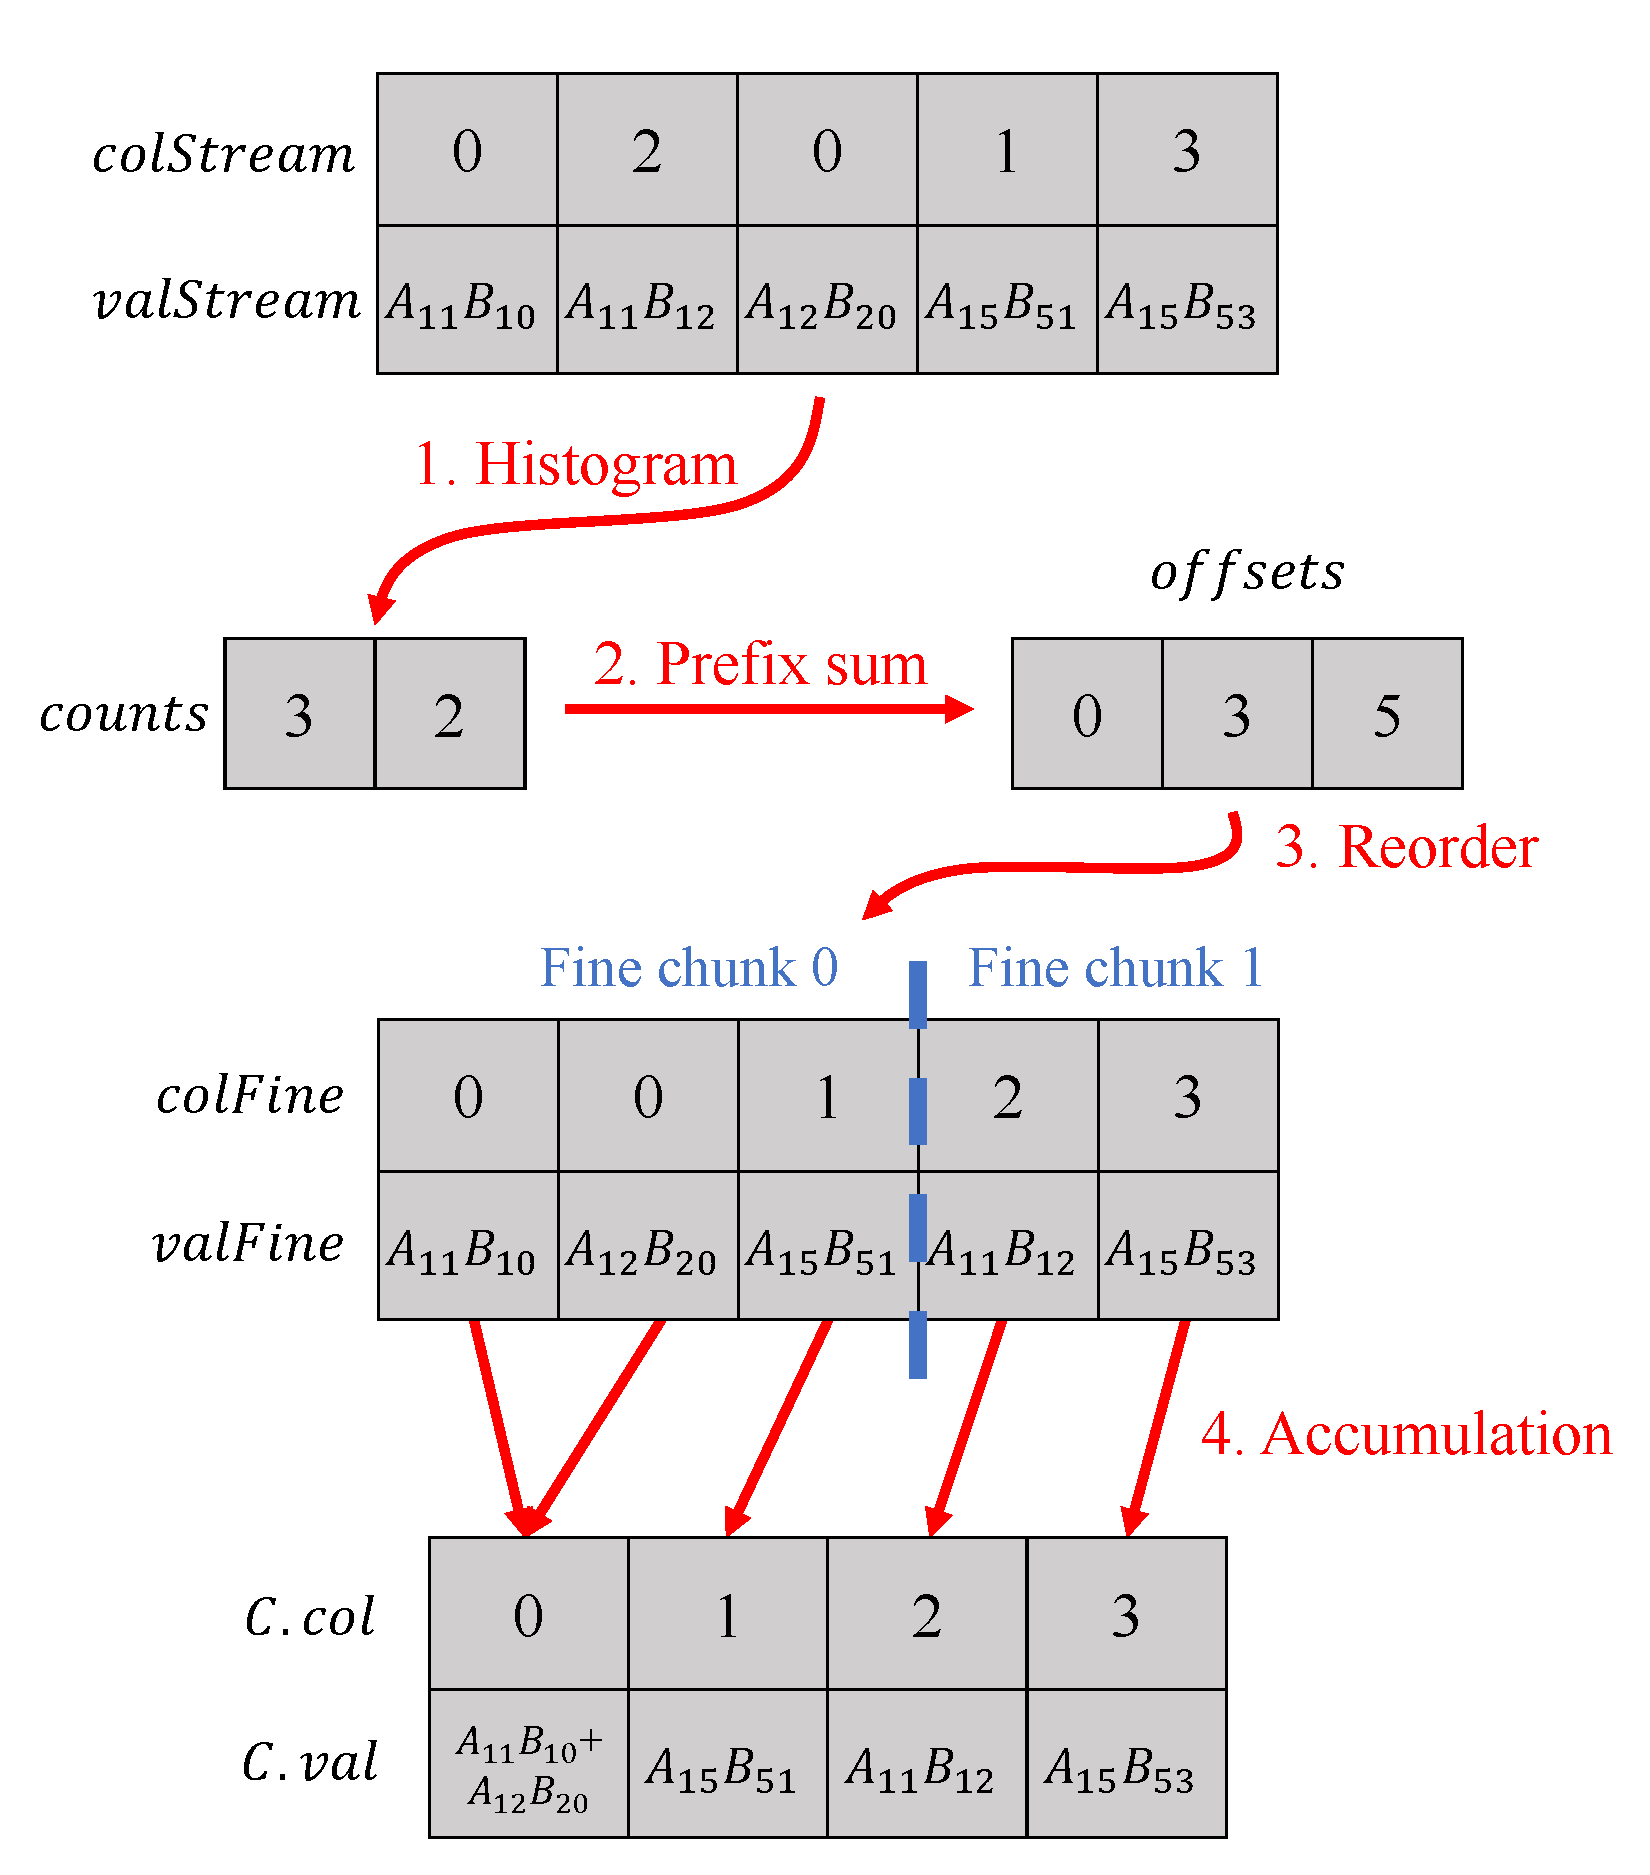
\includegraphics[width=0.61\linewidth]{figs/fineLevel.pdf} 
\end{tabular}
\caption{Data structure-view of applying the fine-level algorithm to the first chunk from \autoref{fig:MAGNUS_example}.}
\label{fig:fineLevel_example}
\end{figure}

The first step towards reordering the intermediate product is to compute $offsetsFine$ (the chunk offsets) using a histogram and a prefix sum operation.  
The array $offsetsFine$ stores the start and end locations of each fine-level chunk in $colFine$ and $valFine$.
The buffers $colFine$ and $valFine$ are typical of any ESC-type algorithm where the intermediate product must be explicitly stored.  In the case of MAGNUS, they store the reordered intermediate product.
In the histogram step, the column indices are mapped to chunks as $col / chunkLenFine$, where $chunkLenFine = m_{C_{maxL2}} / n_{chunksFine}$ is the \textit{chunk length} of the fine-level chunks.
The chunk length is the local range of the column indices within a chunk, where column indices are shifted into the range $[0,chunkLenFine)$ as shown on line 15.
The value of $m_{C_{maxL2}}$ is equal to $m_C$ if the fine-level algorithm is used alone, or equal to the coarse chunk length if the coarse-level algorithm is used ($m_{C_{maxL2}}$ is discussed in more detail in \autoref{sec:magnus_opt_params}).
To optimize the mapping, the division operation is replaced with a bitwise operation by restricting $n_{chunksFine}$ to a power of two, ensuring that $m_C / n_{chunksFine}$ is also a power of two.
Therefore, the mapping becomes $col \texttt{>>} shiftFine$, where $shiftFine = \log_2(chunkLenFine)$ and $\texttt{>>}$ is the bitwise right-shift operator.

After the histogram is computed, the chunk offsets are computed using a prefix sum (inclusive scan) of the histogram.
To reorder the input (shown in the second loop), the histogramming phase is repeated, where the histogram is used to track the current
number of elements in each chunk.
Elements are reordered by writing the input coarse-level chunk at the position $offsetsFine[chunk]+countsFine[chunk]$ in $colFine$ and $valFine$.
As mentioned previously, the column indices are shifted into the local range of each chunk as $col - chunk\times chunkLenFine$ to allow for cache-efficient accumulation.

Finally, a call to \texttt{accum()} for each chunk invokes either sort-based accumulation or dense accumulation, where the size of $denseAccumBuff$ (see \autoref{alg:gustav_dense}) is now reduced from $m_{C_{maxL2}}$ to $chunkLenFine$.
After the accumulation step, the column indices are shifted back into the correct range before writing to $C$.
The variable $rangeFine_j$ denotes the range of column indices of the fine-level chunk $j$ (i.e., $[j\times chunkLenFine,(j+1)\times chunkLenFine)$), and $rangeCoarse$
is the range of column indices of the input coarse-level chunk.
\autoref{fig:fineLevel_example} shows the workflow of the fine-level algorithm in terms of the data structures from \autoref{alg:magnus_fine}, where the input is the first chunk from the example in \autoref{fig:MAGNUS_example}.

\sloppy The fine-level algorithm requires two additional arrays: $countsFine$ and $offsetsFine$, both of size $n_{chunksFine}$. Alongside $denseAccumBuff$ and $bitMap$, the goal is to keep $countsFine$, $offsetsFine$, and the active cache lines of $colFine$ and $valFine$ in the L2 cache.
The active cache lines must be considered since we are writing to $colFine$ and $valFine$ at noncontiguous positions.
In our implementations, we use non-temporal streaming stores when writing to $colFine$ and $valFine$, which avoids polluting the L2 cache.
Non-temporal stores are intrinsic functions used on Intel processors (e.g., \texttt{_mm512\_stream\_si512()}) that write to memory without evicting cached data, allowing us to retain the accumulator and fine-level data structures in the L2 cache while streaming the intermediate product.
\autoref{sec:magnus_opt_params} shows how we choose the optimal number of chunks that minimizes the total storage cost of these cached arrays.

\subsection{The Coarse-level Algorithm}\label{sec:magnus_coarse}
As the columns of $C$ increase, the storage of the fine-level data structures eventually exceeds the size of the L2 cache.
An initial coarse level must be generated for such matrices, providing the first level of locality.
To generate the coarse level, we use a modified outer product-based algorithm, where the intermediate product is generated and reordered for all rows that require coarse-level locality before any accumulation occurs.
The reordered intermediate product is organized into discrete coarse-level chunks that can be handled independently by the fine-level algorithm.

The outer product-based approach is used because the coarse-level algorithm computes only the intermediate product without performing any accumulation.
Therefore, maximizing the reuse of the input matrices rather than the accumulator is beneficial, which is a well-known property of outer product-based SpGEMM algorithms~\cite{pbSpGEMM,gamma}.
The combination of our reordering algorithm with the outer product formulation makes the coarse-level algorithm similar to propagation blocking-based algorithms~\cite{pbSpGEMM}.

Conventional outer product algorithms typically generate the intermediate product by multiplying the columns of $A$, stored in CSC format, with the rows of $B$, stored in CSR format.
The coarse-level algorithm in MAGNUS follows the same scheme, but on the subset of the rows categorized as coarse-level rows.
Therefore, a CSC version of the submatrix $\hat{A}$ of $A$ is constructed, where $\hat{A}$ only includes these coarse-level rows.
Each thread performs the following steps on its list of coarse-level rows, which are stored in the array $coarseRowsC$:
\begin{enumerate}
    \item For all $i\in coarseRowsC$, generate $coarseRowsB$, i.e., the unique set of rows in $B$ required to perform the outer product.  This is done by iterating through the nonzero entries in $\hat{A}$ and setting a bitmap, where $coarseRowsB$ is the list of set bits.
    \item Construct the thread-local CSC submatrix $\hat{A}^{CSC}$ using the well-known approach for the conversion of CSR to CSC: a histogramming stage computes the number of nonzero entries per row, a prefix sum computes $\hat{A}^{CSC}.colPtr$, and $\hat{A}^{CSC}.colPtr$ is then used to construct the arrays $\hat{A}^{CSC}.row$ and $\hat{A}^{CSC}.val$.
    This step is inexpensive since the time complexity of outer product-based SpGEMM algorithms is dominated by the generation of the intermediate product in the following step. Specifically, the time complexity of constructing $\hat{A}$ is $O(nnz_{\hat{A}})$, while generating the intermediate product requires $O(\sum_{(i,j)\in \mathcal{S}(\hat{A})}nnz_{B_j})$ time, which is best-case $O(nnz_{\hat{A}})$ (i.e., each row in $B$ contains only one nonzero value) and worst-case $O(nnz_{\hat{A}} m_B)$ (i.e., each row in $B$ is dense).
    \item Perform a histogram step by reading $\hat{A}^{CSC}$ and the rows of $B$ corresponding to $coarseRowsB$.
    A prefix sum of the resulting histogram generates the coarse-level offsets.
    \item Generate the coarse level by again reading $\hat{A}^{CSC}$, reading the rows of $B$ corresponding to $coarseRowsB$, and writing the result in $colCoarse$ and $valCoarse$ at the positions determined by the offsets.
    As in the fine-level algorithm, we use non-temporal streaming stores for the reordering.
    \item For each coarse-level chunk, apply the fine-level algorithm.
\end{enumerate}

Steps 3-5 are shown in \autoref{alg:magnus_coarse}.
The same set of basic building blocks is used as in the fine-level algorithm (histogramming, prefix summing, and reordering).
The key difference is that the chunks for all rows are generated at the same time.
The prefix sum is modified to compute the chunk offsets within a row based on the offsets from the previous rows.
Just as in the fine-level algorithm, we generate the reordered intermediate product using non-temporal streaming stores.
In the final loop, the fine-level algorithm is applied to each coarse-level chunk for each row.
\autoref{fig:coarseLevel_example} shows the data structures for the example in \autoref{fig:MAGNUS_example}.

\begin{figure}[htbp]
\centering
\begin{tabular}{c}
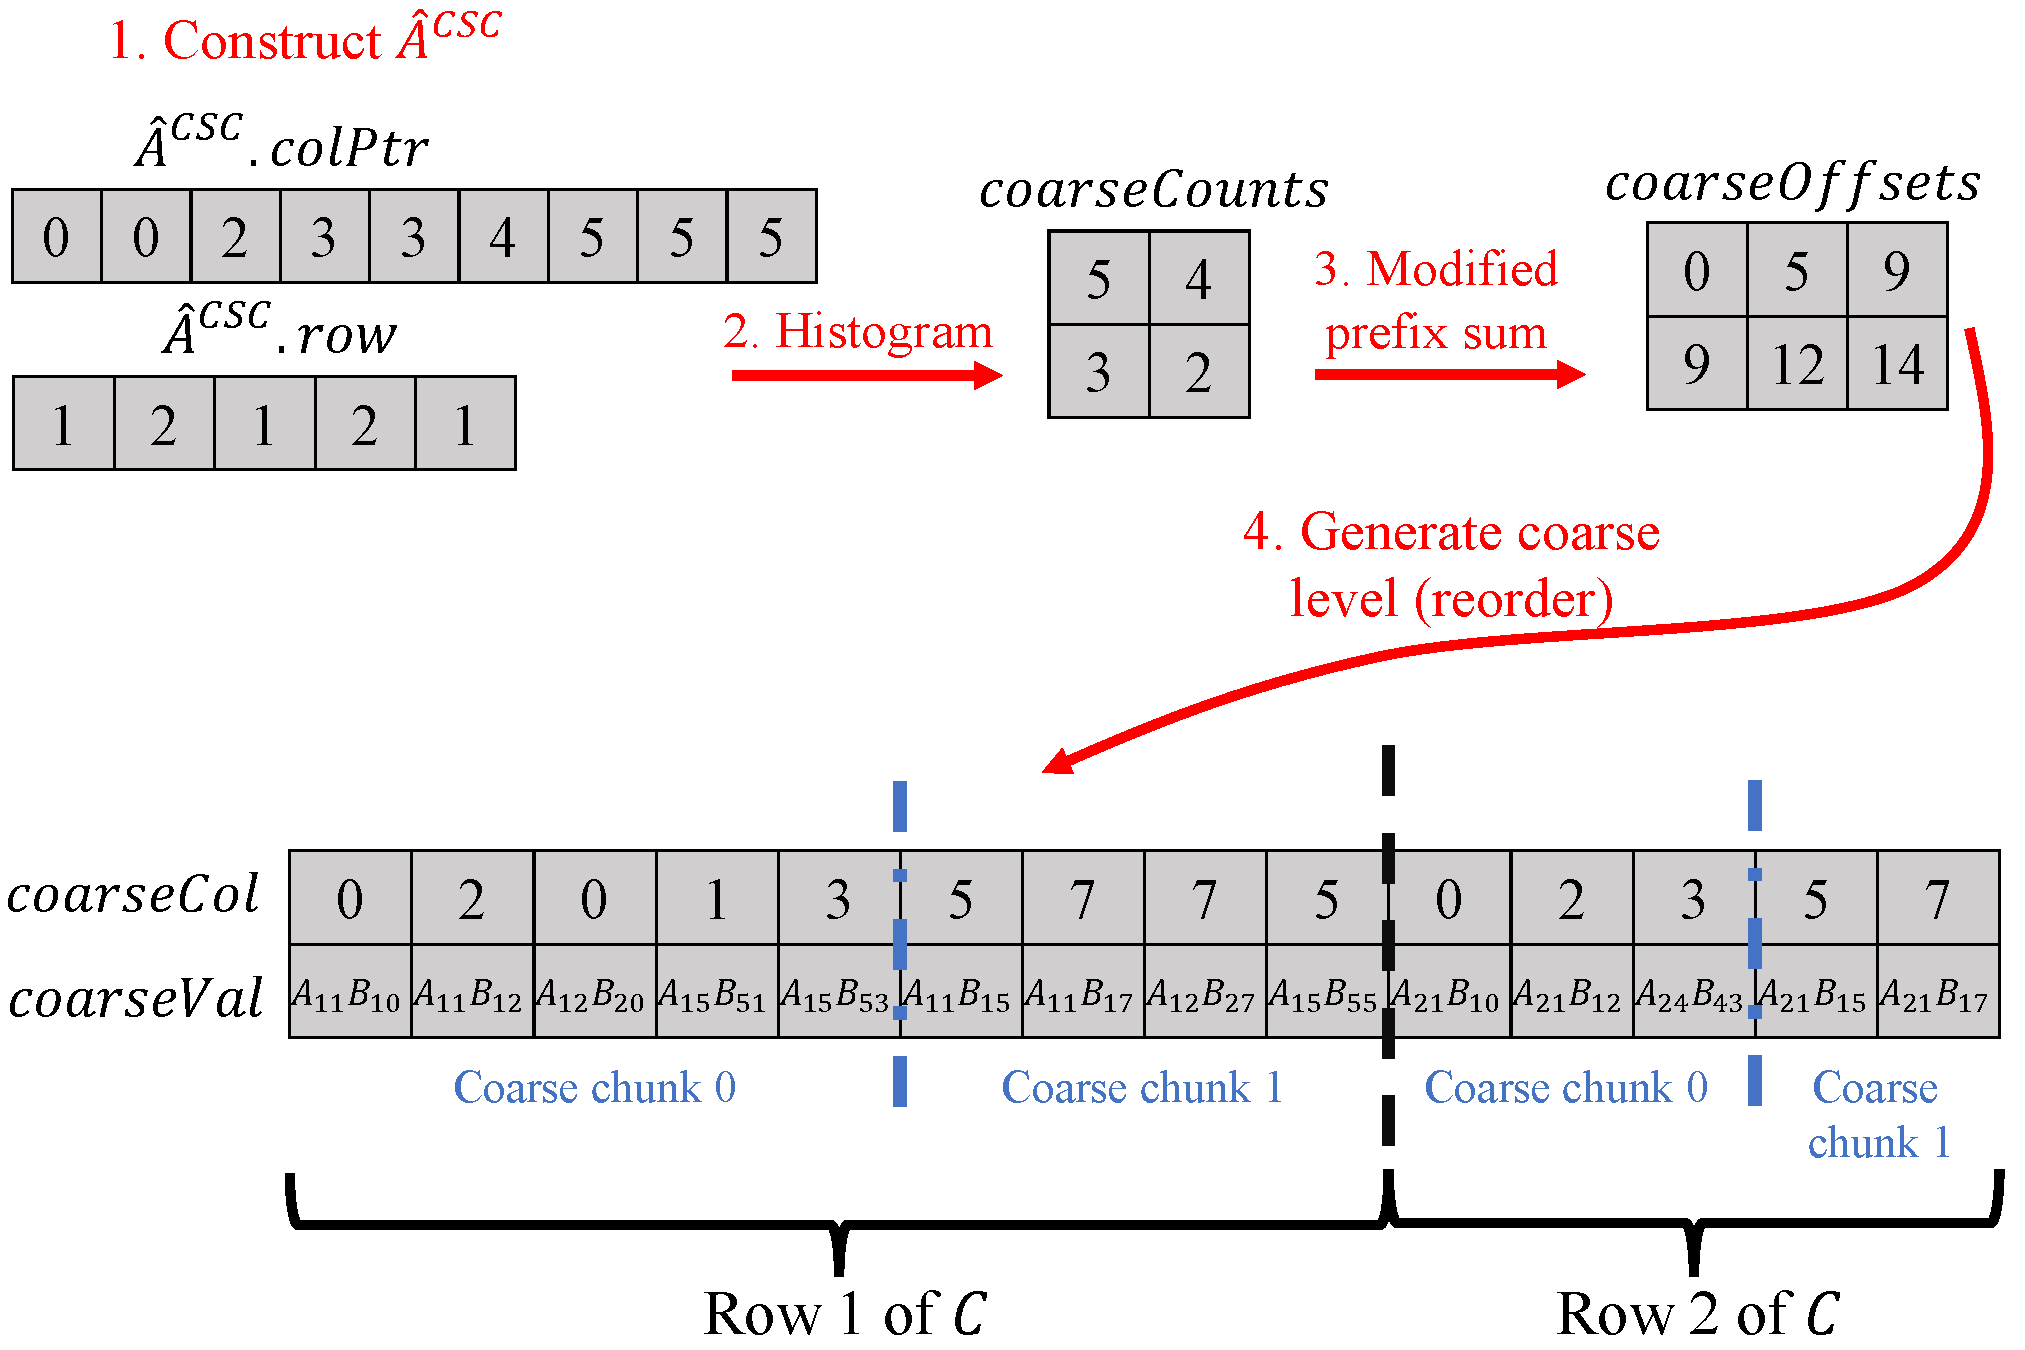
\includegraphics[width=0.9\linewidth]{figs/coarseLevel.pdf} 
\end{tabular}
\caption{Data structure-view of the coarse-level algorithm for the example in \autoref{fig:MAGNUS_example}.}
\label{fig:coarseLevel_example}
\end{figure}


\begin{algorithm}[htbp]
    \small
    \caption{MAGNUS coarse-level algorithm}\label{alg:magnus_coarse}
    \KwIn{$\hat{A}^{CSC}$, $\boldsymbol{B}$, $coarseRowsB$, $coarseRowsC$}
    \KwOut{$\boldsymbol{C}_{coarseRowsC}$}
    \SetCommentSty{emph}
    \DontPrintSemicolon
    $countsCoarse \gets 0$\;
    \text{\textbf{\color{blue}/* Histogram*/}}\;
    \For{$i \in coarseRowsB$}{
        \For{$j \gets \hat{A}^{CSC}.colPtr[i]$\textbf{ to }$\hat{A}^{CSC}.colPtr[i+1]-1$}{
            \For{$k \gets \boldsymbol{B.rowPtr}[i]$\textbf{ to }$\boldsymbol{B.rowPtr}[i+1]-1$}{
                $chunk \gets \boldsymbol{B.col}[k]$\texttt{>>}$shiftCoarse$\;
                $countsCoarse[\hat{A}^{CSC}.row[j]][chunk]$\texttt{++}\;
            }
        }
    }
    \text{\textbf{\color{blue}/* Prefix sum */}}\;
    $offsetsCoarse[0][0] \gets 0$\;
    \For{$i \in coarseRowsC$}{
        $\&offsetsCoarse[i][1] \gets$ \texttt{inclusiveScan(}$countsCoarse[i]$\texttt{)}\;
        $offsetsCoarse[i+1][0] \gets offsetsCoarse[i][n_{chunksCoarse}] $\;
    }
    \text{\textbf{\color{blue}/* Reorder */}}\;
    $countsCoarse \gets 0$\;
    \For{$i \in coarseRowsB$}{
        \For{$j \gets \hat{A}^{CSC}.colPtr[i]$\textbf{ to }$\hat{A}^{CSC}.colPtr[i+1]-1$}{
            \For{$k \gets \boldsymbol{B.rowPtr}[i]$\textbf{ to }$\boldsymbol{B.rowPtr}[i+1]-1$}{
                $chunk \gets \boldsymbol{B.col}[k]$\texttt{>>}$shiftCoarse$\;
                $\ell \gets offsetsCoarse[\hat{A}^{CSC}.row[j]][chunk]+countsCoarse[\hat{A}^{CSC}.row[j]][chunk]$\texttt{++}\;
                $colChunks[\ell] \gets \boldsymbol{B.col}[k]-chunk\times chunkLenCoarse$\;
                $valChunks[\ell] \gets \hat{A}^{CSC}.val[j]\times \boldsymbol{B.val}[k]$\;
            }
        }
    }
    \text{\footnotesize\textbf{\color{blue}/* Apply fine-level algorithm to each coarse-level chunk */}}\;
    \For{$i \in coarseRowsC$}{
        \For{$j \gets 0$\textbf{ to }$n_{chunksCoarse}-1$}{
            $k \gets offsetsCoarse[i][j]$\;
            $\boldsymbol{C}_{i,rangeCoarse_j} \gets$ \texttt{fineLevel(}$\&colCoarse[k],\&valCoarse[k]$\texttt{)}\;
        }
    }
\end{algorithm}

The coarse-level algorithm utilizes a set of data structures similar to that of the fine-level algorithm, but without an accumulator. The absence of a cached accumulator enables the coarse-level algorithm to generate more chunks than the fine-level algorithm. However, this comes at the cost of increased data volume due to the additional pass over the intermediate product.
Despite this tradeoff, for a sufficiently large matrix, the increased data volume proves more efficient than the frequent cache misses incurred by the fine-level algorithm, as we will demonstrate in our microbenchmark results.

Similarly to other outer product-based approaches, the memory requirement for the coarse-level algorithm is higher than the fine-level algorithm since the intermediate product for multiple rows must be stored.
In the worst case, the memory requirement is proportional to the sum of the outer products of all rows, which may exceed the memory capacity of certain memory-constrained systems.
Therefore, we use a batching approach, where we collect rows of $C$ into $coarseRowsC$ until one of two conditions is met:
(1) the memory limit of our system is reached, or (2) the storage requirement for generating the coarse-level chunks ($countsCoarse$, $offsetsCoarse$, and the small buffers for the non-temporal streaming stores) exceeds the L2 cache size.
If either condition is met, the batch of rows in $coarseRowsC$ is computed via steps 2-5.
This batching process is repeated until all rows requiring coarse-level locality have been computed.

\subsection{Accumulation}\label{sec:magnus_accum}
MAGNUS is accumulator-agnostic, allowing for portability and flexibility: only the storage requirements of the desired accumulators
are needed to compute the optimal MAGNUS parameters (the optimal parameters are derived in \autoref{sec:magnus_opt_params}.
For portability, accumulators optimized for specific architectures can be selected without changing the locality-generation algorithms.
This is evident in \autoref{alg:magnus_fine}, where the \texttt{accum()} function requires only an input chunk.
For flexibility, MAGNUS allows for a hybrid approach in which each chunk chooses an accumulator based on the chunk characteristics.
In this paper, we consider two accumulators: AVX-512 vectorized bitonic sorting~\cite{AVX512sort} and classical dense accumulation.
For chunks with a small number of elements, sorting is performed. Otherwise, dense accumulation is used.
When visiting each chunk, a threshold is used to choose the accumulator.
This threshold is based on how the sorting algorithm is implemented: quicksort partitions the array, and then hard-coded, vectorized bitonic sorting networks sort the partitions.
We found experimentally that dense accumulation is faster than sorting unless the sort size is small enough to bypass the quicksort algorithm and directly use bitonic sorting.
For more details, see \autoref{sec:results_sort} and~\cite{AVX512sort}.

\subsection{Choosing the Number of Chunks}\label{sec:magnus_opt_params}

The optimal number of chunks is chosen based on the following input parameters, which are readily available for end users: $s_{cacheLine}$, $s_{L2}$, and $m_C$.
Parameters $s_{cacheLine}$ and $s_{L2}$ are the cache line and L2 cache sizes, respectively, which are retrieved by querying the underlying system, e.g., by using standard Linux commands.
Parameter $m_C$ is the number of columns of $C$, which is already included in the CSR data structure of $B$ since $m_C = m_B$.

As explained in \autoref{sec:magnus_fineLevel}, the goal is to retain in the L2 cache certain data structures needed by the fine-level algorithm.
For simplicity, assume $m_C$ is a power of two ($m_C$ is ceiled to the nearest power of two otherwise).
Choosing the optimal number of fine-level chunks corresponds to selecting the value of $n_{chunksFine}$ that minimizes the convex function
\begin{equation}
s_{fineLevel} = \frac{m_C s_{denseAccum}}{\boldsymbol{n_{chunksFine}}} + \boldsymbol{n_{chunksFine}} s_{chunkFine},
\label{equ:fine_level_storage}
\end{equation}
where $s_{fineLevel}$ is the storage requirement for the L2-cached fine-level data structures.
The first term is the storage requirement of the dense accumulator, where the number of elements in the underlying dense accumulator array is $m_C/n_{chunksFine}$. 
For the numeric phase, $s_{denseAccum} = s_{val}+1$, since we need $denseAccumBuff$ and $bitMap$ (see \autoref{alg:gustav_dense}).
For the symbolic phase, $s_{denseAccum} = 1$ since we only need $bitMap$.
The second term is the storage requirement for reordering,
where the storage cost per fine-level chunk is $s_{chunkFine} = s_{histoType}+s_{prefixSumType}+2 s_{cacheLine}$.
The parameters $s_{histoType}$ and $s_{prefixSumType}$ denote the size of the histogram and prefix sum array data types, respectively, which are both four bytes.
The term $2 s_{cacheLine}$ accounts for the storage of active cache lines when noncontiguously writing to $colFine$ and $valFine$ during the reordering phase.
The value of $n_{chunksFine}$ that minimizes \autoref{equ:fine_level_storage} is
\begin{equation}
\boldsymbol{n_{chunksFine}}=\sqrt{\frac{m_C s_{denseAccum}}{s_{chunkFine}}},
\label{equ:fine_level_nchunks_optimal}
\end{equation}
rounded to the nearest power of two, which
is the number of fine-level chunks used 
when the fine-level algorithm is used alone.

By plugging in $n_{chunksFine}$ from \autoref{equ:fine_level_nchunks_optimal} into \autoref{equ:fine_level_storage} we get
\begin{equation}
s_{fineLevel}=2\sqrt{m_C s_{denseAccum} s_{chunkFine}},
\label{equ:fine_level_storage_optimal}
\end{equation}
which is the total storage requirement of the fine-level algorithm when the optimal number of fine-level chunks is used.
When $m_C$ becomes sufficiently large, $s_{fineLevel}$ exceeds the size of the L2 cache, at which point the coarse-level algorithm is applied.
We can now derive the number of fine- and coarse-level chunks when both levels of locality are used.
In this case, we first determine $m_{C_{maxL2}}$, which is the maximum number of columns in which $s_{fineLevel} \leq s_{L2}$.
To calculate $m_{C_{maxL2}}$, we replace $m_C$ with $m_{C_{maxL2}}$ in \autoref{equ:fine_level_storage_optimal} and solve $s_{fineLevel}=s_{L2}$ for $m_{C_{maxL2}}$.
This gives us
\begin{equation}
m_{C_{maxL2}} = \frac{s_{L2}^2}{4  s_{denseAccum}   s_{chunkFine}},
\label{equ:mCmaxL2}
\end{equation}
which is constant and is floored to the nearest power of two.
Therefore,
\begin{equation}
\boldsymbol{n_{chunksFine}}=\sqrt{\frac{m_{C_{maxL2}} s_{denseAccum}}{s_{chunkFine}}},
\label{equ:fine_level_nchunks_optimal2}
\end{equation}
is the optimal number of fine-level chunks when both levels of locality are used, and
the optimal number of coarse-level chunks is
\begin{equation}
\boldsymbol{n_{chunksCoarse}}=m_C / m_{C_{maxL2}}.
\label{equ:coarse_level_nchunks_optimal}
\end{equation}
Equations~\ref{equ:mCmaxL2} and \ref{equ:fine_level_nchunks_optimal2} show that for a sufficiently large value of $m_C$, the number of fine-level chunks stops growing once the coarse-level algorithm is applied.
At this point, the number of coarse-level chunks begins to grow while maintaining a fixed number of fine-level chunks, ensuring that the fine-level data structures fit into the L2 cache.

Note that we only derive optimal parameters for dense accumulation.
This is because the sort-based accumulator does not require any additional storage since
the arrays storing the intermediate product are directly sorted.
The same analysis can also be applied to other accumulators (e.g., hash maps) by modifying \autoref{equ:fine_level_storage}.